\section{Exclusive distributions}\label{sec:eventselection}

\section{Cuts}

To arrive at a DVEP candidate event, we do the following


Code flow:

Consider a directory with n hipo files. For each hipo file, do the following.

Read each file event by event, and do the following

Check that the event has the proper databanks, and if not, go to teh next event.

Get a list of all the electrons*, protons*, and photons* in the event

*= links to most up to date PID methods

for every electron in the event (always only one, at least in the skims, but not held to be one) do the following
For every proton in the event, do the following

Calculate some basic quantities and fill histograms

for every permutation of pairs of photons in the event, do the following

calculate various kinematic quantities, and pass to see if creates a viable pion* and a viable DVEP event*

if so, fill relevant histograms and count as a DVEP event, otherwise skip to next event

viable pion: 
pion mass betwen 100 and 180 MeV
pion momentum greater than 1.5 GeV
angle (theta) between each photon and the electron to be greater than 8 degrees

viable DVEP event:
Q2 greater than 1
W greater than 2
difference between theta of missing 4-momentum and reconstructed pion less than 2 degrees
difference between missing X px and py 300 MeV each or less
Difference in missing mass squared between pion and X less than 1 GeV ** make sure this is right
difference in missing energy and X less than 1 GeV **make sure this is right

**photon cuts:
pid 22, status > 2000 (in FD or CD, not ftagger)
momentum greater than 400 MeV each

**proton cuts: pid 2212

**electron cuts: pid==1 and status < 0(negative particle

\iffalse
\begin{wrapfigure}{r}{0.58\textwidth}
	\vspace*{-0.3cm}
	\includegraphics[page=10,width=0.97\linewidth]{figures/eppi0.exclusive.pdf}
	\caption{MM$^2$ (epX) vs $\theta_X\pi$ 2D distribution.}
	\label{fig:MM2vsThetaXPi}
\end{wrapfigure}
After the selection of events with at least one electron, proton and two photons, it is time to take a look at the exclusive distributions.
The Fig.~\ref{fig:MM2vsThetaXPi} shows 2D distribution of MM$^2$ (epX) vs $\theta_{X\pi}$, where MM$^2$ (epX) is a missing mass squared of (epX) system and should have a peak near 0.0182 GeV$^2$, and $\theta_{X\pi}$ is an angle between expected and reconstructed pion.
The bright spot on the figure corresponds to the exclusive $ep\rightarrow~ep\pi^0$ events.
In order to reduce the background exclusivity cuts  need to be developed based on the conservation of energy and momentum.
The relevant 1D exclusive distributions are shown on the Fig.~\ref{fig:rawexclusive1} and \ref{fig:rawexclusive2}.

\begin{figure}[hbt]
	\centering
	\includegraphics[page=4,width=0.47\linewidth]{figures/eppi0.exclusive.pdf}
	\includegraphics[page=5,width=0.47\linewidth]{figures/eppi0.exclusive.pdf}

	\caption{Exclusive distributions for events with at least one electron, proton and two photons.}
	\label{fig:rawexclusive1}
\end{figure}

\begin{figure}[hbt]
	\centering
	\includegraphics[page=6,width=0.47\linewidth]{figures/eppi0.exclusive.pdf}
	\includegraphics[page=8,width=0.47\linewidth]{figures/eppi0.exclusive.pdf}
	
	\caption{Exclusive distributions for events with at least one electron, proton and two photons.}
	\label{fig:rawexclusive2}
\end{figure}

\subsection{Tight $M_{\gamma\gamma}$ mass and transverse missing momenta cuts}

The first step is to use tighter $\gamma\gamma$ mass cut: $0.096<M_{\gamma\gamma}<0.168$ GeV, and take a look at the missing transverse momentum distributions (see Fig.~\ref{fig:ptdistributions}).
From momentum conservation law we expect transverse momentum to be zero, so we can apply cuts on $\Delta p_x$ and $\Delta p_y$ to further improve exclusive channel selection.
The cuts $|\Delta p_x|<0.2$ and $|\Delta p_y|<0.2$ correspond roughly to 4-5 $\sigma$.

\begin{figure}[hbt]
	\centering
	\includegraphics[page=24,width=0.47\linewidth]{figures/eppi0.exclusive.pdf}
	\includegraphics[page=25,width=0.47\linewidth]{figures/eppi0.exclusive.pdf}
	
	\caption{Exclusive distributions for events with at least one electron, proton and two photons.}
	\label{fig:ptdistributions}
\end{figure}

The exclusive distributions after tight $M_{\gamma\gamma}$ mass and transverse missing momenta cuts are shown on Fig.~\ref{fig:rawexclusive3} and display much stronger signal peaks on top of reduced background.

\begin{figure}[hbt]
	\centering
	\includegraphics[page=43,width=0.45\linewidth]{figures/eppi0.exclusive.pdf}
	\includegraphics[page=44,width=0.45\linewidth]{figures/eppi0.exclusive.pdf}
	
	\includegraphics[page=45,width=0.45\linewidth]{figures/eppi0.exclusive.pdf}
    \includegraphics[page=47,width=0.45\linewidth]{figures/eppi0.exclusive.pdf}

	\caption{Exclusive distributions after tight $M_{\gamma\gamma}$ mass and transverse missing momenta cuts .}
	\label{fig:rawexclusive3}
\end{figure}

\subsection{$\theta_{X\pi}$ cut determination}

The cut on angle between expected and reconstructed pion is used in order to further reduce background.
To choose the value of the $\theta_{X\pi}$ cut the $MM^2(epX)$ distribution is analyzed at multiple $\theta_{X\pi}$ cut values and fit using gaussian+polynomial function as shown on Fig.~\ref{fig:mm2fordifferenttheta}.
From the fit we can estimate the number of good exclusive events (gaussian) and the number of background events (polynomial) and their dependence on $\theta_{X\pi}$ cut.
Fig.~\ref{fig:sigbgvsthetacutQ2} and~\ref{fig:sigbgvsthetacutxB} show the numbers of signal and background events as functions of $\theta_{X\pi}$ cut value for multiple bins in $Q^2$ and $x_B$.
These plots show that the cut $\theta_{X\pi}<2^\circ$ allows to select the most number of good events with the least background, and relaxing it beyond $2^\circ$ does not gain us any good exclusive events but increases background.


\begin{figure}[hbt]
	\centering
	\includegraphics[page=123,width=0.3\linewidth]{figures/sigbg_eppi0.pdf}
	\includegraphics[page=125,width=0.3\linewidth]{figures/sigbg_eppi0.pdf}
	\includegraphics[page=128,width=0.3\linewidth]{figures/sigbg_eppi0.pdf}
	
	\includegraphics[page=130,width=0.3\linewidth]{figures/sigbg_eppi0.pdf}
	\includegraphics[page=133,width=0.3\linewidth]{figures/sigbg_eppi0.pdf}
	\includegraphics[page=135,width=0.3\linewidth]{figures/sigbg_eppi0.pdf}
	
	\caption{$MM^2(epX)$ distributions for multiple $\theta_{X\pi}$ cut values.}
	\label{fig:mm2fordifferenttheta}
\end{figure}


\begin{figure}[hbt]
	\centering
	
	\includegraphics[width=0.32\linewidth,page=34]{figures/sigbg_eppi0.pdf}
	\includegraphics[width=0.32\linewidth,page=51]{figures/sigbg_eppi0.pdf}
	\includegraphics[width=0.32\linewidth,page=68]{figures/sigbg_eppi0.pdf}
	
	\includegraphics[width=0.32\linewidth,page=85]{figures/sigbg_eppi0.pdf}
	\includegraphics[width=0.32\linewidth,page=102]{figures/sigbg_eppi0.pdf}
	\includegraphics[width=0.32\linewidth,page=119]{figures/sigbg_eppi0.pdf}
	
	\caption{The numbers of signal (red markers) and background (black markers) events as functions of $\theta_{X\pi}$ cut value for multiple $Q^2$ bins.}
	\label{fig:sigbgvsthetacutQ2}
\end{figure}


\begin{figure}[hbt]
	\centering
	
	\includegraphics[width=0.32\linewidth,page=136]{figures/sigbg_eppi0.pdf}
	\includegraphics[width=0.32\linewidth,page=153]{figures/sigbg_eppi0.pdf}
	\includegraphics[width=0.32\linewidth,page=170]{figures/sigbg_eppi0.pdf}
	
	\includegraphics[width=0.32\linewidth,page=187]{figures/sigbg_eppi0.pdf}
	\includegraphics[width=0.32\linewidth,page=204]{figures/sigbg_eppi0.pdf}
	
	\caption{The numbers of signal (red markers) and background (black markers) events as functions of $\theta_{X\pi}$ cut value for multiple $x_B$ bins.}
	\label{fig:sigbgvsthetacutxB}
\end{figure}

\clearpage

\subsection{Final exclusivity cuts}

The list of final exclusive cuts is following:
\begin{itemize}
	\item $\Delta p_x<0.2$ GeV
	\item $\Delta p_y<0.2$ GeV
	\item $\theta_{X\pi}<2^\circ$
	\item $0.096<M_{\gamma\gamma}<0.168$ GeV
	\item $MM^2(epX)<0.5$ GeV$^2$
\end{itemize}

Exclusive distributions after all exclusivity cut except $MM^2(epX)<0.5$ GeV are shown on Fig.~\ref{fig:finalexclusive}

\begin{figure}[hbt]
	\centering
	
	\includegraphics[page=82,width=0.32\linewidth]{figures/eppi0.exclusive.pdf}
	\includegraphics[page=83,width=0.32\linewidth]{figures/eppi0.exclusive.pdf}
	\includegraphics[page=84,width=0.32\linewidth]{figures/eppi0.exclusive.pdf}
	\caption{Exclusive distributions after all exclusivity cuts .}
	\label{fig:finalexclusive}
\end{figure}

\fi